\documentclass{article}

\usepackage{amsmath}
\usepackage{amssymb}
\usepackage{amsthm}
\usepackage{dsfont}
\usepackage{commath}
\usepackage{graphicx}
\usepackage{hyperref}
\usepackage{amsfonts}
\usepackage{bm}

\newcommand{\bba}{{\mathbb A}}
\newcommand{\bbb}{{\mathbb B}}
\newcommand{\bbc}{{\mathbb C}}
\newcommand{\bbd}{{\mathbb D}}
\newcommand{\bbe}{{\mathbb E}}
\newcommand{\bbf}{{\mathbb F}}
\newcommand{\bbg}{{\mathbb G}}
\newcommand{\bbh}{{\mathbb H}}
\newcommand{\bbi}{{\mathbb I}}
\newcommand{\bbj}{{\mathbb J}}
\newcommand{\bbk}{{\mathbb K}}
\newcommand{\bbl}{{\mathbb L}}
\newcommand{\bbm}{{\mathbb M}}
\newcommand{\bbn}{{\mathbb N}}
\newcommand{\bbo}{{\mathbb O}}
\newcommand{\bbp}{{\mathbb P}}
\newcommand{\bbq}{{\mathbb Q}}
\newcommand{\bbr}{{\mathbb R}}
\newcommand{\bbs}{{\mathbb S}}
\newcommand{\bbt}{{\mathbb T}}
\newcommand{\bbu}{{\mathbb U}}
\newcommand{\bbv}{{\mathbb V}}
\newcommand{\bbw}{{\mathbb W}}
\newcommand{\bbx}{{\mathbb X}}
\newcommand{\bby}{{\mathbb Y}}
\newcommand{\bbz}{{\mathbb Z}}

\newcommand{\bma}{{\bm a}}
\newcommand{\bmb}{{\bm b}}
\newcommand{\bmc}{{\bm c}}
\newcommand{\bmd}{{\bm d}}
\newcommand{\bme}{{\bm e}}
\newcommand{\bmf}{{\bm f}}
\newcommand{\bmg}{{\bm g}}
\newcommand{\bmh}{{\bm h}}
\newcommand{\bmi}{{\bm i}}
\newcommand{\bmj}{{\bm j}}
\newcommand{\bmk}{{\bm k}}
\newcommand{\bml}{{\bm l}}
\newcommand{\bmm}{{\bm m}}
\newcommand{\bmn}{{\bm n}}
\newcommand{\bmo}{{\bm o}}
\newcommand{\bmp}{{\bm p}}
\newcommand{\bmq}{{\bm q}}
\newcommand{\bmr}{{\bm r}}
\newcommand{\bms}{{\bm s}}
\newcommand{\bmt}{{\bm t}}
\newcommand{\bmu}{{\bm u}}
\newcommand{\bmv}{{\bm v}}
\newcommand{\bmw}{{\bm w}}
\newcommand{\bmx}{{\bm x}}
\newcommand{\bmy}{{\bm y}}
\newcommand{\bmz}{{\bm z}}

\newcommand{\bmxi}{{\bm \xi}}

\newcommand{\bmA}{{\bm A}}
\newcommand{\bmB}{{\bm b}}
\newcommand{\bmC}{{\bm c}}
\newcommand{\bmD}{{\bm d}}
\newcommand{\bmE}{{\bm e}}
\newcommand{\bmF}{{\bm f}}
\newcommand{\bmG}{{\bm g}}
\newcommand{\bmH}{{\bm h}}
\newcommand{\bmI}{{\bm i}}
\newcommand{\bmJ}{{\bm j}}
\newcommand{\bmK}{{\bm k}}
\newcommand{\bmL}{{\bm l}}
\newcommand{\bmM}{{\bm m}}
\newcommand{\bmN}{{\bm n}}
\newcommand{\bmO}{{\bm o}}
\newcommand{\bmP}{{\bm p}}
\newcommand{\bmQ}{{\bm q}}
\newcommand{\bmR}{{\bm r}}
\newcommand{\bmS}{{\bm s}}
\newcommand{\bmT}{{\bm t}}
\newcommand{\bmU}{{\bm u}}
\newcommand{\bmV}{{\bm v}}
\newcommand{\bmW}{{\bm w}}
\newcommand{\bmX}{{\bm x}}
\newcommand{\bmY}{{\bm y}}
\newcommand{\bmZ}{{\bm z}}

\newcommand{\cala}{{\mathcal A}}
\newcommand{\calb}{{\mathcal B}}
\newcommand{\calc}{{\mathcal C}}
\newcommand{\cald}{{\mathcal D}}
\newcommand{\cale}{{\mathcal E}}
\newcommand{\calf}{{\mathcal F}}
\newcommand{\calg}{{\mathcal G}}
\newcommand{\calh}{{\mathcal H}}
\newcommand{\cali}{{\mathcal I}}
\newcommand{\calj}{{\mathcal J}}
\newcommand{\calk}{{\mathcal K}}
\newcommand{\call}{{\mathcal L}}
\newcommand{\calm}{{\mathcal M}}
\newcommand{\caln}{{\mathcal N}}
\newcommand{\calo}{{\mathcal O}}
\newcommand{\calp}{{\mathcal P}}
\newcommand{\calq}{{\mathcal Q}}
\newcommand{\calr}{{\mathcal R}}
\newcommand{\cals}{{\mathcal S}}
\newcommand{\calt}{{\mathcal T}}
\newcommand{\calu}{{\mathcal U}}
\newcommand{\calv}{{\mathcal V}}
\newcommand{\calw}{{\mathcal W}}
\newcommand{\calx}{{\mathcal X}}
\newcommand{\caly}{{\mathcal Y}}
\newcommand{\calz}{{\mathcal Z}}


\title{Neural Networks: Theory and Practice}
\author{Yu Gai}
\date{}

\DeclareMathOperator{\deg}{deg}
\DeclareMathOperator{\diag}{diag}
\DeclareMathOperator{\range}{range}
\newcommand{\ind}{{\mathds 1}}
\newcommand{\pp}[2]{{\frac{\partial {#1}}{\partial {#2}}}}
\newtheorem{theorem}{Theorem}

\begin{document}

\maketitle

\tableofcontents

\newpage

\section{Multi-layer Perceptron}

\subsubsection{The probably approximately correct (PAC) learning framework}

\begin{itemize}
\item An input space $\calx \subset \bbr^d$
\item An output space $\caly$, either $\{\pm 1\}$ or $\bbr$
\item A probability measure $\bbp$ over $\calx$
\item An unknown mapping $y: \calx \mapsto \caly$
\item An i.i.d. sample $\{(\bmx_i, y_i)\}_{i = 1}^n$, where $\bmx_i \sim \bbp$ and $y_i = y(\bmx_i)$
\end{itemize}

\subsubsection{Empirical risk minimization (ERM)}

Choose a hypothesis $h$ from a hypothesis space $\calh$ by computing
\[
h^* \triangleq \argmin_{h \in \calh} \frac1n \sum_{i = 1}^n \ind_{h(\bmx_i) \ne y_i}
\]
when $\caly = \{\pm 1\}$, or
\[
h^* \triangleq \argmin_{h \in \calh} \frac1n \sum_{i = 1}^n (h(\bmx_i) - y_i)^2
\]
when $\caly = \bbr$.

\subsubsection{The perceptron model}

Consider the case $\caly = \bbr$.
The hypothesis space of perceptrons is
\[
\calh \triangleq \{h_{\bmw, b} : \bmw \in \bbr^d, b \in \bbr\}
\]
where
\[
h_{\bmw, b} (\bmx)
\triangleq \bmw^T \bmx + b
= \sum_{i = 1}^d \bmw_i \bmx_i + b
\]
is a perceptron.
Choose $\bmw$ and $b$ by computing
\begin{align*}
\argmin_{\bmw, b} \ell (\bmw, b)
& = \argmin_{\bmw, b} \frac1n \sum_{i = 1}^n (h_{\bmw, b} (\bmx_i) - y_i)^2 \\
& = \argmin_{\bmw, b} \frac1n \sum_{i = 1}^n (\bmw^T \bmx_i + b - y_i)^2
\end{align*}

\subsubsection{Interpretation of perceptron as neuron}

\begin{figure}
\centering
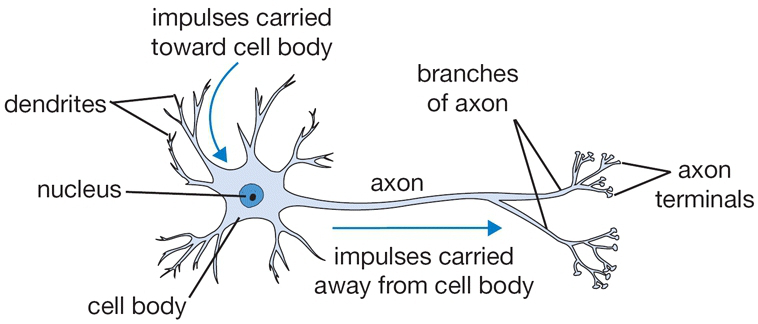
\includegraphics[scale=0.2, valign=t]{neuron}
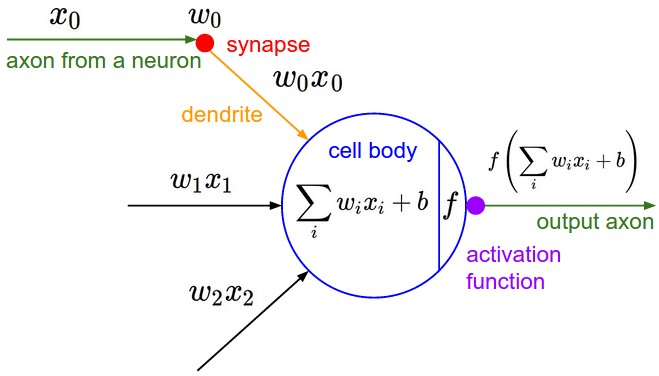
\includegraphics[scale=0.2, valign=t]{neuron_model}
\caption{Analogy between biological neuron and perceptron (figures from \url{http://cs231n.github.io/neural-networks-1/})}
\end{figure}

In the case of perceptron, the activation function is $\sigma (x) = x$.
Other choices of $\sigma$:
\[
\sigma (x) = \frac1{1 + \exp (-x)} \qquad
\sigma (x) = \tanh (x) \qquad
\sigma (x) = \max (0, x)
\]

\subsubsection{The limitation of perceptron: learning the \textsc{XOR} operation}

Consider the case $\calx = \caly = \{0, 1\}$, $\bbp$ is uniform over $\calx$, and
\[
y(\bmx)
= y(x_1, x_2)
= \textsc{XOR} (x_1, x_2) \triangleq \ind_{x_1 = x_2}
\]
\[
\{((0, 0), 1), ((1, 0), 0), ((0, 1), 0), ((1, 1), 1)\} \subset \{0, 1\}^2 \times \{0, 1\}
\]
$\bmw = (w_1, w_2) \subset \bbr^2$
\[
h_{\bmw, b} (\bmx) = w_1 x_1 + w_2 x_2 + b
\]
\[
\argmin_{w_1, w_2, b} \ell (\bmw, b) = ?
\]

Solution: ``linear" combination of neurons with nonlinear activation function.

\[
g(\bmx) = \sum_{i = 1}^{d_1} v_i h_{\bmw_i, b_i} (\bmx) + a
\]
where
\[
h_{\bmw, b} (\bmx) = \sigma(\bmw^T \bmx + b)
\]
and $\bmw_i$ and $b_i$ are the weight and bias of the $i$th neuron.

Interpretation: a perceptron taking as input the activation of other neurons.

\begin{figure}
\centering
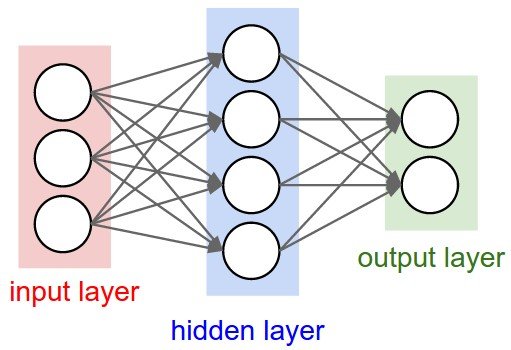
\includegraphics[scale=0.2, valign=t]{neural_net}
\caption{A neural network with one hidden layer (figure from \url{http://cs231n.github.io/neural-networks-1/})}
\end{figure}

\subsubsection{Vectorization}

More compactly,
\[
g(\bmx)
= \sum_{i = 1}^{d_1} v_i h_{\bmw_i, b_i} (\bmx) + a
= \bmv^T \sigma (W \bmx + \bmb) + a
\]
where $\bmv = [v_1, ..., v_{d_1}]$, the $i$th row of $W \in \bbr^{d_1 \times d}$ is $\bmw_i$, and $\bmb = [b_1, ..., b_{d_1}]^T$.
For $\bmv \in \bbr^d$ and $\sigma: \bbr \mapsto \bbr$,
\[
\sigma (\bmv) \triangleq [\sigma (v_1), ..., \sigma (v_d)]^T
\]
$\sigma (W \bmx + \bmb)$ is the activation of the hidden layer because $\sigma (W \bmx + \bmb)_i$ is the activation of the $i$th neuron.

\subsubsection{High-dimensional output}

Replace $\bmv \in \bbr^{d_1}$ by $V \in \bbr^{d_1 \times d_2}$ and $a \in \bbr$ by $\bma \in \bbr^{d_2}$ if $\caly \subset \bbr^{d_2}$:
\[
g(\bmx) = V \sigma (W \bmx + \bmb) + \bma
\]
Interpretation: multiple perceptrons taking as input the activation of a collection of neurons (the $i$th row of $V$ and $a_i$ are the weight and bias of the $i$th perceptron).

\subsubsection{Multi-layer perceptron (MLP)}

Replace input layer by hidden layer, i.e. $\bmx$ by $\sigma (W \bmx + \bmb)$, again, again, and again \ldots
\begin{align*}
\bmh_0 & = \bmx \\
\bmh_i & = \sigma (W_i \bmh_{i - 1} + \bmb_i) \qquad i = 1, ..., L - 1 \\
g(\bmx) & = W_L \bmh_{L - 1} + \bmb_L
\end{align*}
where $h_i$ is the activation of the $i$th hidden layer.

\begin{figure}
\centering
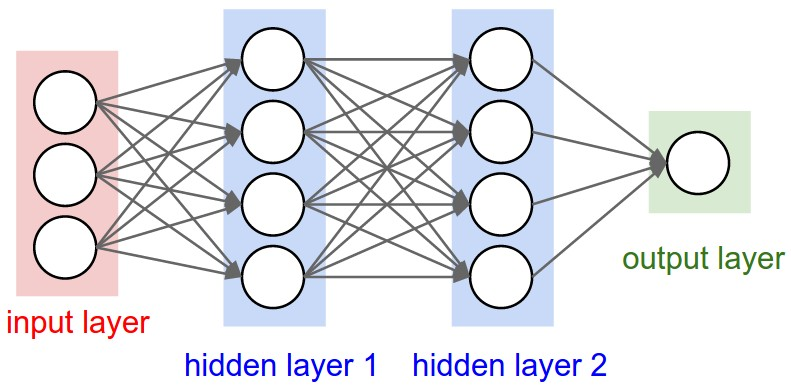
\includegraphics[scale=0.2, valign=t]{neural_net2}
\caption{An MLP with two hidden layers (figure from \url{http://cs231n.github.io/neural-networks-1/})}
\end{figure}

\subsubsection{The universal approximator theorem}

Let $\calh_{NN} \triangleq \{\text{neural network with one hidden layer}\}$.
$\calh_{NN}$ is a hypothesis space much richer than the space of perceptrons:
\begin{theorem}[\cite{cybenko1989approximation}]
$\calh_{NN}$ is dense in $C ([0, 1]^d)$.
\end{theorem}

There is no free lunch!
PAC-learnability lost:
\begin{corollary}
\[
d_{VC} \left(\left\{\ind_{h(\cdot) > \frac12} : h \in \calh_{NN}\right\}\right) = \infty
\]
\end{corollary}
Essentially a consequence of the universal approximator theorem and the fact that $C ([0, 1]^d)$ shatters any finite subset of $[0, 1]^d$.

\subsubsection{VC-dimension and PAC-learnability}

\begin{definition}
The \emph{VC-dimension} of a hypothesis space $\calh$ is defined as
\[
d_{VC} (\calh) \triangleq \max \{n : \Pi_\calh (n) = 2^n\}
\]
where for $n \in \bbn$,
\[
\Pi_\calh (n) \triangleq \max_{\{x_i\}_{i = 1}^n \subset \calx} |\{h(x_i)\}_{i = 1}^n : h \in \calh\}|
\]
\end{definition}

$\calh$ shatters $\{x_i\}_{i = 1}^n$ if $|\{h(x_i)\}_{i = 1}^n : h \in \calh\}| = 2^n$.
The VC-dimension of $\calh$ is the greatest $n$ such that $\calh$ shatters some subset of size $n$.

\begin{theorem}
\[
d_{VC} (\calh) < \infty
\Leftrightarrow \calh\ \text{is PAC-learnable (by ERM)}
\]
\end{theorem}

\subsubsection{Sketched proof of infinite VC-dimension}

It suffices to prove that $\left\{\ind_{h(\cdot) > \frac12} : h \in \calh_{NN}\right\}$ shatters any finite subset of $[0, 1]^d$.
$\forall n \in \bbn$, $\forall E \triangleq \{x_i\}_{i = 1}^n \subset [0, 1]^d$, $\forall F \subset E$, $\exists f \in C([0, 1]^d)$ s.t.
\[
f(F) = \{1\} \qquad f(E - F) = \{0\}
\]
Because $\calh_{NN}$ is dense in $C([0, 1]^d)$, $\forall \epsilon > 0$, $\exists h \in \calh_{NN}$ s.t.
\[
\sup_{\bmx \in [0, 1]^d} |f(\bmx) - h(\bmx)| < \epsilon
\]
In particular, $\exists h \in \calh_{NN}$ s.t.
\[
\max_{\bmx \in E} |f(\bmx) - h(\bmx)| < \frac14
\]

\subsubsection{Solution to lost PAC-learnability: structural risk minimization (SRM) \cite{vapnik1992principles}}

Motivation:
\begin{theorem}
Suppose $d_{VC} (\calh) < \infty$.
Then with probability at least $1 - \eta$,
\[
\forall h \in \calh, R (h) < \hat{R} (h) + \delta_\calh
\]
where
\[
\delta_\calh \triangleq \sqrt{\frac{d_{VC} (\calh) \left(\log \frac{2 n}{d_{VC} (\calh)} + 1\right) - \log \eta}{n}}
\]
\end{theorem}

\subsubsection{Structural risk minimization (continued)}

Suppose $\exists \calh_1 \subset \calh_2 \subset ...$ such that
\[
\calh = \bigcup_i^\infty \calh_i
\]
Let $h_i^* \triangleq \argmin_{h \in \calh_i} \hat{R} (h)$.
It follows that
\[
\hat{R} (h_1^*) \leq \hat{R} (h_2^*) \leq \ldots \qquad
\]
Also,
\[
d_{VC} (\calh_1) \leq d_{VC} (\calh_2) \leq \ldots
\Rightarrow \delta_{\calh_1} \geq \delta_{\calh_2} \geq \ldots
\]

Hopefully the upper bound $\hat{R}(h_i^*) + \delta_{\calh_i}$ is a U-shaped function of $i$ (analoguous to bias-variance trade-off).

\subsubsection{Structural risk minimization (continued)}

How to optimize a U-shaped function of one integer variable?

Let $U(i) \triangleq \hat{R}(h_i^*) + \delta_{h_i}$.
\begin{algorithmic}
\STATE $i \gets 1$
\WHILE{$U(i) \leq U(i + 1)$}
    \STATE $i \gets i + 1$
\ENDWHILE
\RETURN $i$
\end{algorithmic}

Algorithmically, SRM is feasible as long as ERM is feasible, i.e. it is feasible to compute $h_i^*$.

\subsubsection{SRM applied to $\calh_{NN}$}

Let $\calh_{NN}^n \triangleq \{\text{neural network with one hidden layer of size}\ n\}$.
\[
\calh_{NN} = \bigcup_{n = 1}^\infty \calh_{NN}^n
\]

Each $\calh_{NN}^n$ is a more restricted hypothesis space:
\begin{theorem}[\cite{maass1995vapnik}]
If $\sigma (x) = 1 / (1 + \exp (-x))$, then
\[
d_{VC} (\calh_{NN}^n) = \calo (m^4)
\]
where $m$ is the number of weights.
\end{theorem}

Consequence: neural networks with a fixed architecture is PAC-learable, and are not universal function approximators.
Gradient descent.

\subsubsection{SRM applied to $\calh_{NN}$ (continued)}

Apply SRM to the hypothesis familiy
\[
\calh_{NN}^1, \calh_{NN}^2, \ldots
\]
(although it is not the case that $\calh_{NN}^1 \subset \calh_{NN}^2 \subset \ldots$, why?)

It remains to compute
\[
h_i^* \triangleq \argmin_{h \in \calh_i} \hat{R} (h)
\]

\subsubsection{ERM with gradient descent}

As illustrated in class, fix $\calh_{NN}^i$ we can optimize
\[
\frac1n \sum_{i = 1}^n \ell(g(\bmx_i), y_i)
\]
with gradient descent for ``nice" surrogate loss functions $\ell$, although the optimization problem now is always non-convex.

However, you can still give it a try!

We can use the chain rule to compute gradient (a.k.a. backward propagation).
Hopefully you have mastered the chain rule by now. If not \ldots

\subsubsection{Limitation of SRM}

Approximation complexity:
``[B]esides a negligible set, all functions that can be implemented by a deep network of polynomial size, require exponential size in order to be realized (or even approximated) by a shallow network."\cite{cohen2016expressive}

Consider neurons $\{f_{\bmw, b}\}$ a basis indexed by $\bmw \in \bbr^d$ and $b \in \bbr$.
A complete basis can have high approximation complexity for some functions.

Forget about \emph{universal} approximators and instead look for ``good" (in the language of mathematicians) bases/(in the language of alchemists) architectures!

What does ``good" mean?

\subsubsection{Convolutional neural networks (CNN) for image classification}

An image is a mapping $f: \bbr^2 \rightarrow \bbr^C$ with compact support, where $C$ is the number of channels ($C = 1$ for grayscale image, $C = 3$ for RBG image).

Assume the support is $[0, 1]^2$.

After discretizing $[0, 1]^2$: $\bmx \in \bbr^{W H C}$.

\subsubsection{Fourier transform essentials}

\begin{definition}
The Fourier transform $\calf f$ of $f \in L^1 (\bbr^d)$ is defined as
\[
(\calf f) (\bmxi) \triangleq \int_{\bbr^d} e^{-i \bmxi^T \bmx} f(\bmx) \dif \bmx
\]
The inverse Fourier transform $\calf f$ of $f \in L^1 (\bbr^d)$ is defined as
\[
(\calf f) (\bmx) \triangleq \int_{\bbr^d} e^{i \bmx^T \bmxi} f(\bmxi) \dif \bmxi
\]
\end{definition}

\subsubsection{Fourier transform essentials (continued)}

$L^2 (\bbr^d)$ is a Hilbert space when equipped with the inner product
\[
\langle f, g\rangle_{L^2 (\bbr^d)} \triangleq \int_{\bbr^d} f \bar{g} \dif \mu \qquad \forall f, g \in L^2 (\bbr^d)
\]
where $\mu$ denotes the Lebesgue measure of $\bbr^d$.

\begin{theorem}[Plancherel]
\[
\langle f, g\rangle_{L^2 (\bbr^d)} = \frac1{(2 \pi)^d} \langle \calf f, \calf g\rangle_{L^2 (\bbr^d)} \qquad \forall f, g \in L^1 (\bbr^d) \cap L^2 (\bbr^d)
\]
\end{theorem}

Fact: $L^1 (\bbr^d) \cap L^2 (\bbr^d)$ is dense in $L^2 (\bbr^d)$.

Consequence: $\calf f$ for $f \in L^2 (\bbr^d) - L^1 (\bbr^d)$ can be defined as the limit of
\[
\{\calf f_n\}_{n = 1}^\infty \subset L^1 (\bbr^d) \cap L^2 (\bbr^d)
\]
where $f_n \rightarrow f$ and all convergence is in norm.

\subsubsection{Convolution}

The convolution $k * f$ of $f \in L^1 (\bbr^d) \cap L^2 (\bbr^d)$ with $k \in L^1 (\bbr^d) \cap L^2 (\bbr^d)$ is defined as
\[
(k * f) (\bmy) \triangleq \int_{\bbr^d} k(\bmy - \bmx) f(\bmx) \dif \bmx
\]
where $f$ is interpreted as a signal (e.g. an image), and $k$ is interpreted as a kernel.

\begin{theorem}
\[
k * f = \calf^{-1} ((\calf k) \cdot (\calf f))
\]
\end{theorem}

Interpretation: filtering in the Fourier domain.

\subsubsection{Discretized convolution}

\begin{figure}
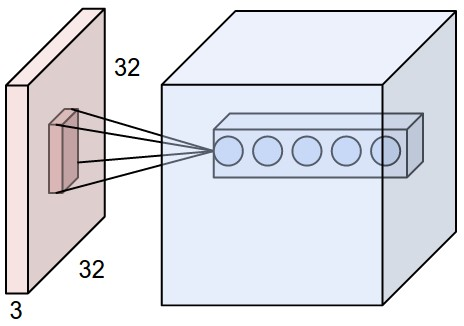
\includegraphics[scale=0.2]{depthcol}
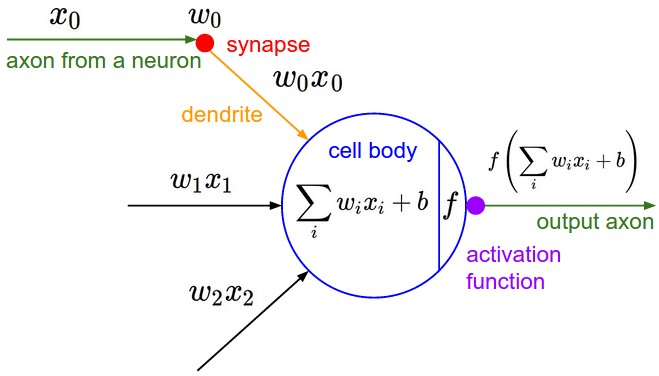
\includegraphics[scale=0.2]{neuron_model}
\caption{Convolution (figure from \url{http://cs231n.github.io/convolutional-networks/})}
\end{figure}

\subsubsection{Downsampling tricks}

\begin{figure}
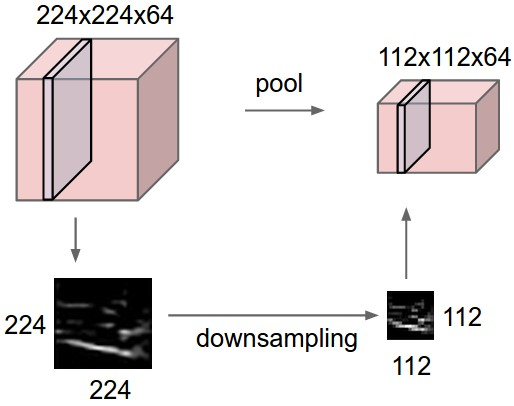
\includegraphics[scale=0.2]{pool}
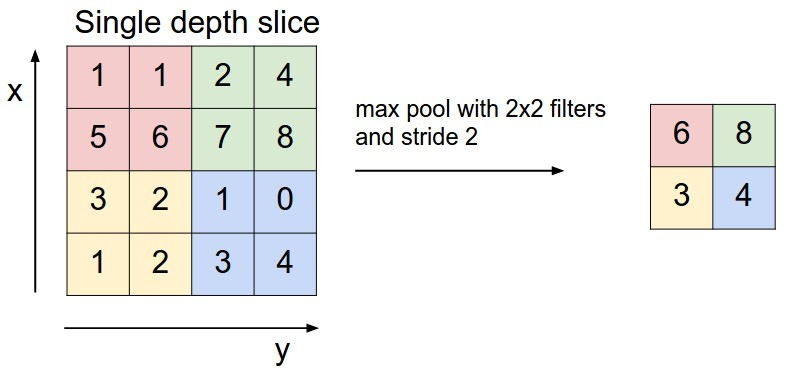
\includegraphics[scale=0.2]{maxpool}
\caption{Pooling (figure from \url{http://cs231n.github.io/convolutional-networks/})}
\end{figure}

\subsubsection{Example: LeNet}

\begin{figure}
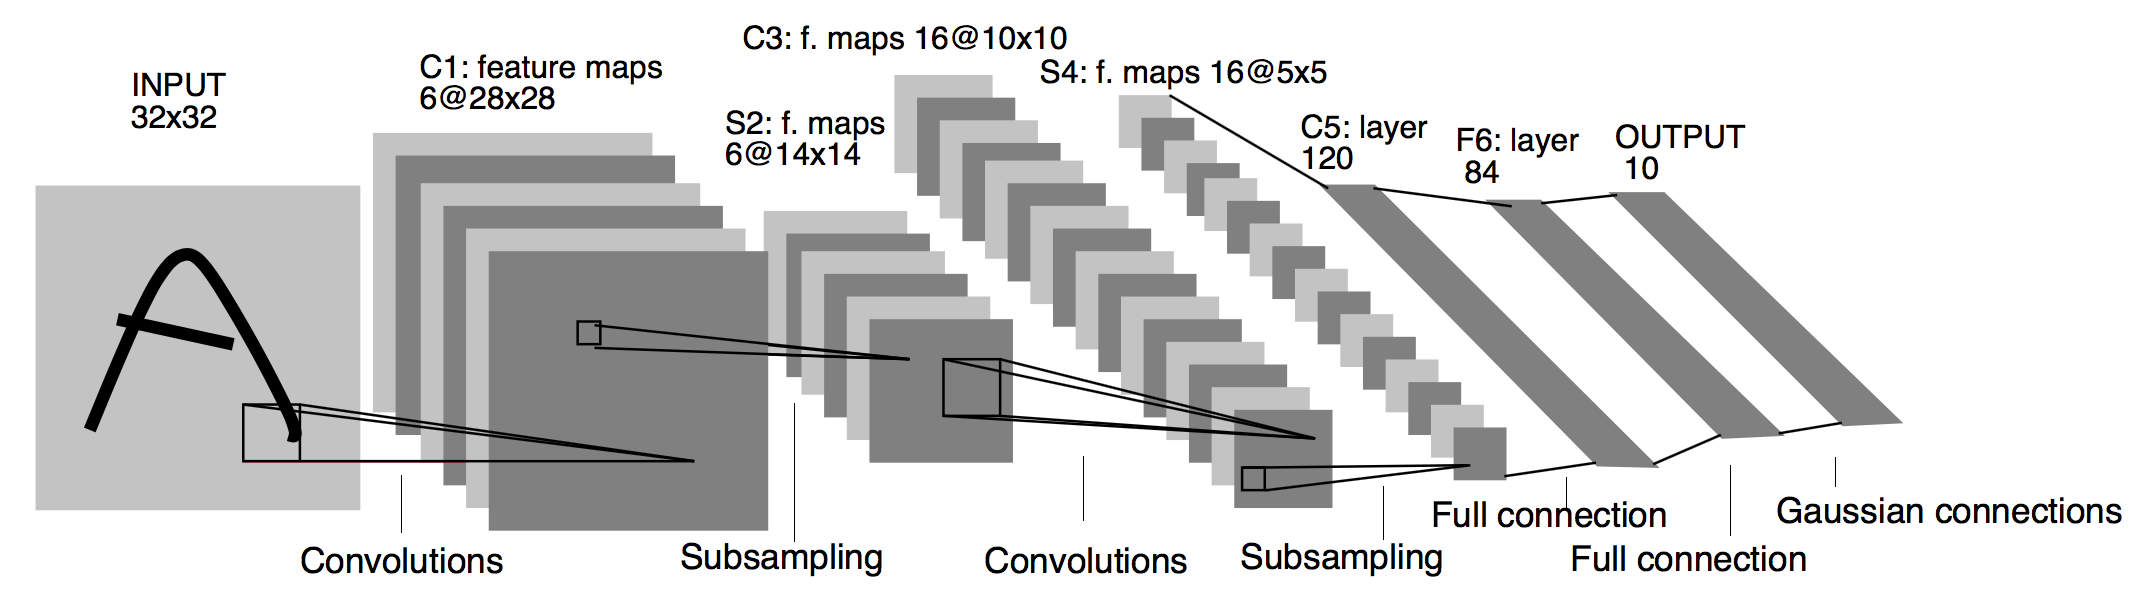
\includegraphics[scale=0.1]{lenet}
\caption{The architecture of LeNet (figure from \cite{lecun1998gradient})}
\end{figure}

\subsubsection{Invariance}

Displacement/Deformation field:
\[
\tau: \bbr^d \mapsto \bbr^d \in \calc^2
\]
Displacement/Deformation operator:
\[
(\call_\tau f) (\bmx) \triangleq f(\bmx - \tau (\bmx))
\]
Example (translation):
\[
\tau (\bmx) = \bmc \qquad
(\call_\tau f) (\bmx) = f(\bmx - \bmc)
\]

\subsubsection{Translation invariance}

Convolution is translation invariant because
\begin{align*}
(k * (\call_\tau f)) (\bmy)
& = \int_{\bbr^d} k(\bmx) (\call_\tau f) (\bmy - \bmx) \dif \bmx \\
& = \int_{\bbr^d} k(\bmx) f(\bmy - \bmx - \bmc) \dif \bmx \\
& = \int_{\bbr^d} k(\bmx) f((\bmy - \bmc) - \bmx) \dif \bmx \\
& = (k * f) (\bmy - \bmc) \\
& = (\call_\tau (k * f)) (\bmy)
\end{align*}

Why is MLP not translation invariant?

Open question: for what kind of kernels is convolution deformation-invariant?

\subsubsection{The belief in information bottleneck}

\cite{mallat2012group} shows how to construct a deformation-invariant kernel.

However, is it the best kernel?

Learning with information bottleneck may result in better kernels.

An early success of neural networks was the perceptron, an affine
\[
f(x) = w^T x \qquad w \in \bbr^d
\]
However,

\subsection{Forward and Backward Propagation}

Given an input $x \in \bbr^d$, the forward propagation rule of a $L$-layer perceptron with weights $\{W^{(l)}\}_{l = 1}^L$, biases $\{b_l\}_{l = 1}^L$, and activation function $\sigma: \bbr \mapsto \bbr$ is defined as
\begin{alignat*}{2}
h_0 & \triangleq x \\
\bar{h}_l & \triangleq W^{(l)} h_{l - 1} + b_l && \qquad l \in [L - 1] \\
h_l & \triangleq \sigma (\bar{h}_l) && \qquad l \in [L - 1] \\
h_L & \triangleq W^{(L)} h_{L - 1} + b_L
\end{alignat*}
where $[n] \triangleq \{1, ..., n\}$, $W^{(l)} \in \bbr^{d_l \times d_{l - 1}}$ with $d_0 \triangleq d$, $b_l \in \bbr^{d_l}$, and the application of $\sigma$ is pointwise.
Typical choices of $\sigma$ are the logistic function $\sigma (\cdot) = \frac1{1 + \exp (-\cdot)}$, the hyperbolic tangent $\sigma = \tanh$, and the rectified linear unit (ReLU) $\sigma (\cdot) = \max (0, \cdot)$.

Given a supervision signal $y \in \caly$ and a loss function $\ell: \bbr^{d_L} \times \caly \mapsto \bbr$, backward propagation refers to the computation of $\{W^{(l)}'\}_{l = 1}^L$ and $\{\pp{\ell}{b_l} (h_L, y)\}$, where $W_{i j}^{(l)}' \triangleq \pp{\ell}{W_{i j}^{(l)}} (h_L, y)$
it follows from the chain rule that the corresponding backward propagation rule is
\begin{alignat*}{2}
h_L' & \triangleq \nabla_{h_L} \ell (h_L, y) \\
W^{(L)}' & \triangleq \nabla_{W^{(L)}} \ell (h_L, y) = h_L' h_{L - 1}^T \\
b_L' & \triangleq \nabla_{b_L} \ell (h_L, y) = h_L' \\
h_{L - 1}' & \triangleq \nabla_{h_{L - 1}} \ell (h_L, y) = W^{(L) T} h_L' \\
\bar{h}_l' & \triangleq \nabla_{\bar{h}_l} \ell (h_L, y) = \diag (\sigma' (\bar{h}_l)) h_{l + 1}' && \qquad l \in [L - 1] \\
W^{(l)}' & \triangleq \nabla_{W^{(l)}} \ell (h_L, y) = \bar{h}_l' h_{l - 1}^T && \qquad l \in [L - 1] \\
b_l' & \triangleq \nabla_{b_l} \ell (h_L, y) = \bar{h}_l' && \qquad l \in [L - 1] \\
h_l' & \triangleq \nabla_{h_l} \ell (h_L, y) = W^{(l) T} \bar{h}_l' && \qquad l = 0, ..., L - 2
\end{alignat*}
where $\diag (x)_{i j} \triangleq x_i \delta_{i j}$ and the application of $\sigma'$ is again pointwise.

\subsection{Approximation theorems}

Let $I_d \triangleq [0, 1]^d$ and let $C (I_d)$ be the space of continuous functions on $I_d$.

\begin{theorem}[\cite{cybenko1989approximation}]
$2$-layer perceptrons with logistic activation function are dense in $C (I_d)$.
\end{theorem}

\begin{theorem}
$2$-layer perceptrons with logistic activation function are dense in $L^1 (I_d)$.
\end{theorem}

\begin{theorem}
$2$-layer perceptrons with logistic activation function are dense in $L^2 (I_d)$.
\end{theorem}

\subsection{The VC-dimension of multi-layer perceptrons}

\subsection{Empirical risk minimization with stochastic gradient descent}

\section{Neural networks for structured data}

Structured data refers to data representable as a mapping $\Omega \mapsto \bbr^d$.
For example, in the case of sequential/temporal data, $\Omega$ is real intervals representing time;
in the case of image data, $\Omega$ is rectangles in $\bbr^2$;
in the case of graph data, $\Omega$ is a graph.

\subsection{Recurrent neural networks: neural networks for sequential/temporal data}

An example of sequential data is sentences in natural languages.
A natural motivation for the architecture of recurrent neural network (RNN) is the following.
Suppose we are trying to evaluate the probability for a sequence $\{x_t\}_{t = 1}^T \subset \bbr^d$ to occur.
It follows from the definition of conditional probability that
The motivation for RNN is to summarize $\{X_s = x_s : s < t\}$, i.e. the conditions at time $t$, by a vector $h_t \in \bbr^H$, and approximate.
The simplest
\[
W_x x + W
\]
\[
\bbp (X_1 = x_1, ..., X_T = x_T)
= \prod_{t = 1}^T \bbp (X_t = x_t | X_s = x_s\ \text{for}\ s < t)
\]
It is crucial that the number of parameters in recurrent neural networks is independent from the sequence length $T$, which enables RNN's to handle long sequences.
The performance of RNN depends significantly on how well the vector $h_t$ summarizes the conditions at time $t$.
It turns out that the simplest RNN can easily "forget" conditions in distant past.
One possible remedy is the long short term memory (LSTM) network, defined as
\begin{align*}
f_t & = \sigma (W_f x_t + U_f h_{t - 1} + b_f) \\
i_t & = \sigma (W_i x_t + U_i h_{t - 1} + b_i) \\
o_t & = \sigma (W_o x_t + U_o h_{t - 1} + b_o) \\
c_t & = f_t \odot c_{t - 1} + i_t \odot \sigma_c (W_c x_t + U_c h_{t - 1} + b_c) \\
h_t & = o_t \odot \sigma_h (c_t)
\end{align*}
where $\odot$ denotes the Hadamard product, $\sigma$ denotes the sigmoid function, $\sigma_c = \tanh$, and $\sigma_h$ is either $\tanh$ or the identity function.
$f$, $i$, and $o$ respectively refer to the forget gate, input gate, and output gate.
The heuristic of LSTM is to control how the internal state $c$ is forgot, enriched, and output by gating.
A simplification of LSTM is the gated recurrent unit (GRU), defined as
\begin{align*}
z_t & = \sigma (W_z x_t + U_z h_{t - 1} + b_z) \\
r_t & = \sigma (W_r x_t + U_r h_{t - 1} + b_r) \\
h_t & = (1 - z_t) \odot h_{t - 1} + z_t \sigma_h (W_h x_t + U_h (r_t \odot h_{t - 1}) + b_h)
\end{align*}
where $z$ and $r$ refer to the update and reset gate.

\subsection{Principles of geometric deep learning}

a.k.a. geometric deep learning.

\subsection{Basics of harmonic analysis}

Given $f \in L^1 (\bbr^d)$, the Fourier transform of $f$ is defined as
\[
(\calf f) (\xi) = \int_{\bbr^d} e^{-i \xi x} f(x) \dif x
\]
It follows that $\calf f \in L^\infty (\bbr^d)$ for $f \in L^1 (\bbr^d)$ because
\begin{align*}
\sup_{\xi \in \bbr^d} |(\calf f) (\xi)|
& = \sup_{\xi \in \bbr^d} \left|\int_{\bbr^d} e^{-i \xi x} f(x) \dif x \right| \\
& \leq \sup_{\xi \in \bbr^d} \int_{\bbr^d} \left|e^{-i \xi x} f(x) \right| \dif x \\
& = \sup_{\xi \in \bbr^d} \int_{\bbr^d} |f(x)| \dif x \\
& = |f|_{L^1 (\bbr^d)}
\end{align*}
where $\sup$ denotes the essential supremum, as in the definition of $L^\infty (\bbr^d)$.

A fundamental property of the Fourier transform is that smoothness in the spatial domain implies decay in the frequency domain.
To state it in a general setting, we introduce the following definitions.
Given a $d$-dimensional multi-index $\alpha = (\alpha_1, ..., \alpha_d) \in \bbn^d$, the differential operator $D^\alpha$ is defined as
\[
D^\alpha \triangleq \frac{\partial^{\alpha_1}}{\partial x_1^{\alpha_1}} \cdot \ldots \cdot \frac{\partial^{\alpha_d}}{\partial x_d^{\alpha_d}}
\]
The order $|\alpha|$ of $\alpha$ is defined as
\[
|\alpha| \triangleq \sum_{i = 1}^d \alpha^i
\]
Define
\[
\calc^k \triangleq \{f : D^\alpha f\ \text{is continuous for all}\ |\alpha| \leq k\}
\]
We restrict $D^\alpha$ to $\calc^{|\alpha|}$, so that the ordering of partial differential operators in the definition of $D^{\alpha}$ does not matter by Schwarz's theorem.
For $1 \leq p \leq \infty$ and $k \in \bbn$, the ($L^p$)-Sobolev space of order $k$ is defined as
\[
W_p^k \triangleq \{f \in L^p : D^\alpha f \in L^p\ \text{for all}\ |\alpha| \leq k\}
\]
Stoke's theorem states that
\[
\int_\Omega \dif \omega = \int_{\partial \Omega} \omega
\]

The Laplacian is defined as
\[
\Delta \triangleq \sum_{i = 1}^d \frac{\partial^2}{\partial x_i^2}
\]
For a function $u: \bbr^{d + 1} \mapsto \bbr$, where the first $d$ dimensions are spatial and the last dimension is temporal, the heat equation is
\[
\pp{u}{t} = c \Delta u
\]

\subsection{Deep learning on images}

\subsubsection{Non-parametric convolutional neural networks}

It turns out that for some simple tasks, e.g. MNIST digit recognition, convolutional neural networks without learnable parameters can achieve state of the art performance as well.
In the following we describe the architecture of PCANet \cite{chan2015pcanet}, a convolutional neural network with filters inferred solely from Principle Component Analysis (PCA).
Consider a dataset consisting of $n$ image-label pairs
\[
\{(x_i, y_i)\}_{i \in [n]} \subset \bbr^{W H C} \times \caly
\]
where $W$, $H$, and $C$ are the width, height, and number of channels of images, and $\caly$ is the collection of labels.
Suppose the filter (patch) $W$ has size $k_w \times k_h$.
The parameters of the filter is computed by applying PCA to the vectors
\[
\bigcup_{i = 1}^n \{x_{i, j}\}_{j = 1}^{k_w k_h}
\]
where $x_{i, pq}$ denotes the $k_w \times k_h$ patch with top left corner located at pixel $(p, q)$ of image $x_i$.
Suppose the number of output channels is $C'$.
Then retain the leading $C'$ eigenvectors of the corresponding covariance matrix as filter.
Such "PCAConv" layers can be cascaded.
Once complete,

\subsection{Deep learning on graphs}

In the following we describe neural networks tailored to data with graph structures.
More precisely, we are interested in data representable as $\calv \mapsto \bbr^d$ for some graph $\calg = (\calv, \cale)$.
We shall assume that both $\calv$ and $\cale$ are finite and adopt the convention that $n \triangleq |\calv|$ and $m \triangleq |\cale|$.
We shall identify $\calv$ with $[n]$ and $\cale$ with $[m]$.
We assume that $\calg$ is undirected, i.e. $(i, j) \in \cale \Leftrightarrow (j, i) \in \cale$ for all $i, j \in \calv$.
We assume that $\calg$ has no self-connection, i.e. $(i, i) \ne \cale$ for $i \in [n]$.
Let $M_i$ denote the $i$-th row of $M$, and $M^i$ denote the $i$-th column of $M$.

\subsubsection{Laplacian on graphs}

A real-valued function (signal) on $\calg = (\calv, \cale)$ is a mapping $\calv \mapsto \bbr$, which can be identified with a vector in $\bbr^n$ by identifying $\calv$ with $[n]$.
We assume that along with $\calg$ comes a real symmetric matrix $W$ and $W_{i j}$ is a positive number interpreted as the strength of connection between $i, j \in \calv$.
The degree of $i \in \calv$ is defined as
\[
\deg (i) \triangleq \sum_{j = 1}^n W_{i j}
\]
and the degree matrix $D$ of $\calg$ is an $n \times n$ diagonal matrix defined as
\[
D_{i j} \triangleq \delta_{i j} \deg (i)
\]
The Laplacian of $\calg$ is defined as
\[
L \triangleq D - W
\]
An alternative motivation for the definition of graph Laplacian is the following.
Suppose $u: \calv \times \bbr \mapsto \bbr$ describes the evolution of heat distribution over $\calv$.
Newton's law of cooling states that the heat transferred between $i, j \in \calv$ in an infinitestimal period of time is proportional to the difference $u_i - u_j$ when $(i, j) \in \cale$.
Consequently,
\begin{align*}
\pp{u_i}{t}
& = -c \sum_{(i, j) \in \cale} w_{i j} (u_i - u_j) \\
& = -c \left(\deg (i) u_i - \sum_{(i, j) \in \cale} w_{i j} u_j\right)
\end{align*}
Vectorizing the identity, we have
\begin{align*}
\pp{u}{t}
& = -c (D u - A u) \\
& = -c (D - A) u \\
& = -c L u
\end{align*}

\subsubsection{Convolution on graphs}

\begin{equation*}
f * g (x) \triangleq \int_{\bbr^d} f(y) (\calt_x (\calr g)) (y) dy
\end{equation*}
where $(\calr g) (\cdot) \triangleq g(-\cdot)$ is the reflection operator and $(\calt_x g) (\cdot) \triangleq g(x + \cdot)$ is the translation (by $x$) operator.
Neither $\calr$ nor $\calt_x$ makes sense when we replace $\bbr^d$ by $\calg$.
\begin{equation*}
f * g = \calf^{-1} (\calf  f \calf g)
\end{equation*}

Other definitions of Laplacian exists in the literature.
For example, the random walk Laplacian is defined as
\[
L^{RW} \triangleq I - W D^{-1}
\]
However, the random walk Laplacian is in general asymmetric and thus unsuitable for our purpose.
It follows from the spectral theorem for real symmetric matrix that $L$ admits the decomposition
\begin{equation*}
L = U^T \Lambda U
\end{equation*}
where $U \in SO(n)$, $L U_i = \Lambda_{i i} U_i$ for $i \in [n]$, $\Lambda$ is diagonal, and $\Lambda_{i i} \leq \Lambda_{j j} \forall 1 \leq i < j \leq n$.
\begin{equation*}
(U f)_i
= f^T U_i
= <f, U_i>_{\bbr^b}
\end{equation*}
which is analoguous to
\begin{equation*}
(\calf f) (n)
\triangleq \int_T e^{-i n x)} f(x) \dif x
= <e^{-i n \cdot}, f>_{L^2}
\end{equation*}
We can define Fourier transform $\calf$ on $\calg$ analoguously as
\begin{equation*}
\calf f \triangleq U f
\end{equation*}
Because $U^T U = I$ on $\bbr^n$ and $\calf^{-1} \calf = I$ on $L^2$, a natural definition for inverse Fourier transform on $\calg$ is
\begin{equation*}
\calf^{-1} \triangleq U^T
\end{equation*}

\begin{equation*}
f * g
\triangleq \calf^{-1} (\calf f \cdot \calf g)
= U^T (U f \odot U g)
\end{equation*}
where $\odot$ denotes the Hadamard product.
Analoguous to the approach to convolution on image, one of $f$ and $g$ filter and the other signal.
In the following let $x$ denote a signal and $\theta$ denote a filter.
\[
\theta * x
= U^T (U \theta \odot U x)
\]
Because $U \in SO(n)$,
\[
\theta * x
= U^T (\theta \odot U x)
= U^T (\diag (\theta) U x)
\]
(possibly with nonlinearity attached)

However, this construction has two disadvantages.
First,
Second, computing the eigen-decomposition $U^T \Lambda U$ is expensive.
One solution, proposed by \cite{defferrard2016convolutional}, is to replace $\diag (\theta)$ with a polynomial of $\Lambda$ with learnable coefficient.
Suppose $\Theta = \sum_{k = 0}^K \theta_k \Lambda^k$.
\begin{align*}
\Theta * x
& = U^T \Theta U x \\
& = U^T \left(\sum_{k = 0}^K \theta_k \Lambda^k \right) U x \\
& = \left(\sum_{k = 0}^K \theta_k U^T \Lambda^k U \right) x \\
& = \sum_{k = 0}^K \theta_k L^k x
\end{align*}
where the last identity follows from the fact that
\[
L L
= U^T \Lambda U U^T \Lambda U
= U^T \Lambda^2 U
\]
It follows from the definition of $L$ that $L$ contains $n + 2 m$ non-zero entries, which is significantly less than $n^2$ when $\calg$ is sparse, i.e. when $m / n^2 \rightarrow 0$.
An efficient implementation of $L x$, commonly referred to as Sparse Matrix-Vector multiplication (SpMV), only requires $\calo ()$ time.
The choice
\[
\Theta = 
\]
results in the popular Graph Convolutional Network (GCN) \cite{kipf2016semi}.

\subsubsection{Spectral clustering revisited}

In the following we describe a neural network architecture motivated by an improved spectral clustering algorithm.

A natural setting for theoretical analysis of spectral clustering algorithms is the Stochastic Block Model (SBM).
In the binary case, given a collection of nodes $\calv = [n]$ and a label assignment $\sigma: \calv \mapsto {\pm 1}$, the probability for two nodes $i, j \in \calv$ to be connected is
\[
\bbp [(i, j) \in \cale]
= \ind_{\sigma_i = \sigma_j} p_{in} + \ind_{\sigma_i \ne \sigma_j} p_{out}
\]
where $p_{in}$ denotes the probability of an inter-community edge and $p_{out}$ denotes the probability of an extra-community edge.
To model sparse graphs, let
\[
p_{in} = \frac{c_{in}}n \qquad
p_{out} = \frac{c_{out}}n
\]
where $c_{in}$ and $c_{out}$ are constants, and $n \rightarrow \infty$.
detectability threshold:
\[
c_{in} - c_{out}
\]
SBM can model many real world graphs, in particular, social networks.
"Birds of a feather flock together."
Importantly, many real world graphs have bounded maximum degree when $n \rightarrow \infty$, i.e.
\[
d^* \triangleq \lim_{n \rightarrow \infty} \max_{i \in \calv} \deg (i) < \infty
\]
These graphs are sparse because
\[
\frac{m}{n^2}
\leq \frac{d^* n}{n^2}
= \frac{d^*}n
\]

It turns out that standard spectral clustering fails at the limit $n \rightarrow \infty$ even if detectable.

\section{Optimization of neural networks}

\subsection{Stochastic gradient descent}

\subsection{A toy example}

In the following we present the results of \cite{le1991eigenvalues}.
Consider the dataset
\[
\{(x_i, y_i)\}_{i = 1}^n \subset \bbr^d \times \bbr
\]
a linear "neural network"
\[
f(x) = w^T x \qquad w \in \bbr^{d}
\]
and the mean square error as objective
\[
\ell (w) = \sum_{i = 1}^n (f(x_i) - y_i)^2
\]
It follows from linear algebra manipulations that
\begin{align*}
\ell (w)
& = \frac1n \sum_{i = 1}^n (f(x_i) - y_i)^2 \\
& = \frac1n \sum_{i = 1}^n (w^T x_i - y_i)^2 \\
& = \frac1n \sum_{i = 1}^n (w^T x_i - y_i) (x_i^T w - y_i) \\
& = \frac1n \sum_{i = 1}^n w^T x_i x_i^T w - 2 y_i w^T x_i + y_i^2 \\
& = w^T \left(\frac1n \sum_{i = 1}^n x_i x_i^T\right) w - \frac{2 w^T}n \sum_{i = 1}^n y_i x_i + \frac1n \sum_{i = 1}^n y_i^2 \\
& = w^T R w - 2 w^T q + c
\end{align*}
where
\[
R \triangleq \frac1n \sum_{i = 1}^n x_i x_i^T
\]
is the sample covariance matrix and
\[
q \triangleq \frac1n \sum_{i = 1}^n y_i x_i
\]
Because
\[
\nabla_w \ell (w) = 2 R w - 2 q
\]
the critical points are solution to the linear system
\[
R w = q
\]
Because $R$ is a square matrix, $R$ is injective if and only if $R$ is surjective.
It follows that when $R$ is injective, $q \in \range R$ and the solution is unique.
Otherwise, it may be the case that either $q \not \in \range R$, or
% argmin?
The corresponding Hessian is
\[
H (w) = 2 R
\]
The sample covariance matrix $R$ is real symmetric and thus has the eigen-decomposition
\[
R = U^T \Lambda U
\]
where $\Lambda$ is diagonal and the rows of $U$ is an orthonormal basis of $\bbr^d$.
In the basis, 

\subsection{The challenge of saddle points}

It turns out that compared with encountering local minima, it is significantly more likely to encounter saddle points if one applies SGD to neural networks.
The following is several related results.

\bibliographystyle{unsrt}
\bibliography{written}

\end{document}
